% A second definition of "usage" inside an experiment, versus one imported definition.
% Colours come from src/styles/palette.json via the generated ../_palette.tex (npm run tokens).
% Shared house style for the TikZ diagrams. render.sh defines \theme (light|dark) before \input.
\documentclass{article}
\usepackage{fontspec}
\usepackage{tikz}
\usepackage{fontawesome5}
\usetikzlibrary{positioning,calc,arrows.meta,fit,backgrounds}
\setmainfont{CrimsonPro}[Path=\fontdir, Extension=.ttf, UprightFont=*, ItalicFont=*-Italic, UprightFeatures={RawFeature={+wght=400}}, ItalicFeatures={RawFeature={+wght=400}}, BoldFont=*, BoldFeatures={RawFeature={+wght=600}}, Scale=1.08]
\setmonofont{JetBrainsMono}[Path=\fontdir, Extension=.ttf, Scale=0.86]
\newfontfamily\kickerfont{JetBrainsMono}[Path=\fontdir, Extension=.ttf, Scale=0.72, LetterSpace=12]
% GENERATED from src/styles/palette.json by scripts/tokens/build.mjs. Do not edit; run `npm run tokens`.
\def\darktheme{dark}
\ifx\theme\darktheme
  \definecolor{ink}{HTML}{EFEFE8}
  \definecolor{muted}{HTML}{A0A09A}
  \definecolor{paper}{HTML}{1B1B19}
  \definecolor{accent}{HTML}{5FE08F}
  \definecolor{accentfill}{HTML}{173322}
  \definecolor{oxide}{HTML}{FF6A4D}
\else
  \definecolor{ink}{HTML}{111111}
  \definecolor{muted}{HTML}{4A4A4A}
  \definecolor{paper}{HTML}{FFFFF8}
  \definecolor{accent}{HTML}{1F7A45}
  \definecolor{accentfill}{HTML}{E6F1EA}
  \definecolor{oxide}{HTML}{C8361C}
\fi

\tikzset{
  every picture/.style={line cap=round, line join=round, font=\normalsize, text=ink},
  card/.style={draw=ink!70!paper, line width=0.6pt, fill=paper, rounded corners=3pt, align=left,
               text width=#1, inner xsep=7pt, inner ysep=5.5pt, anchor=north west},
  card/.default=3.9cm,
  hot/.style={card=#1, draw=accent, line width=1.1pt, fill=accentfill},
  hot/.default=3.9cm,
  ghost/.style={card=#1, draw=muted!80!paper, dashed, fill=none, text=muted},
  ghost/.default=3.9cm,
  panel/.style={draw=muted!45!paper, line width=0.5pt, rounded corners=5pt, inner sep=9pt},
  hotpanel/.style={panel, draw=accent!75!paper, line width=0.9pt},
  line/.style={-{Stealth[length=5pt,width=4.2pt]}, line width=0.7pt, draw=ink!70!paper},
  hotline/.style={line, draw=accent, line width=1pt},
  ghostline/.style={line, draw=muted!80!paper, dashed},
  badline/.style={line, draw=oxide, line width=1pt},
  lbl/.style={font=\small\itshape, text=muted, inner sep=2.5pt},
  head/.style={font=\itshape, text=muted, anchor=south west, inner sep=0pt, align=left},
  warm/.style={card=#1, draw=accent!60!paper, fill=accentfill!50!paper},
  warm/.default=3.9cm,
}
\newcommand{\kicker}[1]{{\kickerfont\MakeUppercase{#1}}}
\newcommand{\ico}[1]{\makebox[1.25em][l]{#1}}
\newcommand{\cardtext}[2]{{\ttfamily #1}\\[1pt]{\small\itshape\color{muted}#2}}
% Crop the page to the picture: typeset it into a box and ship that box as the page.
\newcommand{\diagram}[1]{%
  \setbox0\hbox{#1}%
  \pagewidth=\dimexpr\wd0+8pt\relax \pageheight=\dimexpr\ht0+\dp0+8pt\relax
  \hoffset=-1in \voffset=-1in
  \shipout\vbox{\kern4pt\hbox{\kern4pt\box0}}}

\begin{document}
\diagram{\begin{tikzpicture}[x=1cm,y=1cm]
  \def\tw{3.9cm}
  \def\A{0}\def\B{5.75}\def\C{11.5}
  % ---- what happened
  \node[head, anchor=south west] (h1) at (0,1.0) {\kicker{what happened}\\[3pt] two definitions of the same thing};
  \node[card=\tw, anchor=west] (src) at (\A,0) {\cardtext{src/moseq\_bxd/usage.py}{defines syllable\_usage()}};
  \node[card=\tw, anchor=west] (a) at (\B,0) {\cardtext{\faIcon{flask}\ exp-0009}{imports it}};
  \node[card=\tw, anchor=west] (ua) at (\C,0) {usage = share of\\ syllable instances};
  \node[ghost=\tw, anchor=west] (b) at (\B,-1.75) {\cardtext{\faIcon{flask}\ exp-0014/run.py}{its own compute\_usage()}};
  \node[ghost=\tw, anchor=west] (ub) at (\C,-1.75) {usage = share of\\ frames};
  \node[lbl, anchor=east, align=right] (why) at ($(b.west)+(-0.45,0)$) {a new session didn't\\ look in src/};
  \draw[line] (src) -- node[lbl, above] {import} (a);
  \draw[line] (a) -- (ua);
  \draw[ghostline] (why) -- (b);
  \draw[ghostline] (b) -- node[lbl, above] {rewrote it} (ub);
  \draw[badline, {Stealth[length=5pt,width=4.2pt]}-{Stealth[length=5pt,width=4.2pt]}] (ua) -- node[lbl, text=oxide, right] {\faIcon{not-equal}\ disagree} (ub);
  \begin{scope}[on background layer]
    \node[panel, fit={(h1) (-0.1,-2.6) (16.4,0.5)}] {};
  \end{scope}
  % ---- the rule
  \begin{scope}[yshift=-5.0cm]
  \node[head, text=accent, anchor=south west] (h2) at (0,0.75) {\kicker{the rule}\\[3pt] one definition, imported everywhere};
  \node[hot=\tw, anchor=west] (src2) at (\A,-0.875) {\cardtext{src/moseq\_bxd/usage.py}{defines syllable\_usage(), tested}};
  \node[card=\tw, anchor=west] (a2) at (\B,0) {\cardtext{\faIcon{flask}\ exp-0009}{imports it}};
  \node[card=\tw, anchor=west] (b2) at (\B,-1.75) {\cardtext{\faIcon{flask}\ exp-0014}{imports it}};
  \node[hot=\tw, anchor=west] (u2) at (\C,-0.875) {same usage,\\ everywhere};
  \draw[hotline] (src2.east) -- node[lbl, text=accent, above, sloped] {import} (a2.west);
  \draw[hotline] (src2.east) -- node[lbl, text=accent, below, sloped] {import} (b2.west);
  \draw[hotline] (a2.east) -- (u2.west);
  \draw[hotline] (b2.east) -- (u2.west);
  \node[lbl, anchor=north west, align=left] at (\A,-2.7) {\faIcon{search}\ \ {\upshape\ttfamily just check} flags a function body copied out of src/ (a real rewrite, with a new definition, needs a test that pins it down)};
  \begin{scope}[on background layer]
    \node[hotpanel, fit={(h2) (-0.1,-3.25) (16.4,0.5)}] {};
  \end{scope}
  \end{scope}
\end{tikzpicture}}
\end{document}
